\documentclass[conference]{IEEEtran}
\IEEEoverridecommandlockouts
% The preceding line is only needed to identify funding in the first footnote. If that is unneeded, please comment it out.
\usepackage{cite}
\usepackage{amsmath,amssymb,amsfonts}
\usepackage{algorithmic}
\usepackage{graphicx}
\usepackage{textcomp}
\usepackage{xcolor}
\def\BibTeX{{\rm B\kern-.05em{\sc i\kern-.025em b}\kern-.08em
    T\kern-.1667em\lower.7ex\hbox{E}\kern-.125emX}}
\begin{document}

\title{Detecting Surgeon Stress from ECG Signals: Comparing a 1D CNN
With and Without CBAM Attention on the WESAD Dataset}

\author{
\IEEEauthorblockN{Aly Ayman Zoweil, Mostafa Nader, Abdallah Amr, Asser Mohamed}
\IEEEauthorblockA{\textit{College of Engineering and Technology} \\
\textit{Arab Academy for Science, Technology and Maritime Transport (AASTMT)} \\
Alexandria, Egypt \\
}
}

\maketitle

\begin{abstract}
During high-risk keyhole and robotic surgery, a surgeon under heavy stress can
narrow their attention so much that they miss important cues. This is called
cognitive tunneling. Because the surgeon's hands and eyes are busy with the
instruments, we cannot ask them to enter anything, so we instead try to read
their stress level from their heart signal (the ECG), which changes when a
person becomes stressed. We use the WESAD dataset, which contains chest ECG
recorded at 700~Hz from 15 subjects, and we treat the problem as a two-class
task: baseline (calm) versus stress. A stress prediction is what would raise a
high-stress alert in the real system. We normalize the ECG separately for each
subject, cut it into 10-second windows, and feed the raw windows directly into
a 1D convolutional neural network (CNN) with large kernels and residual
connections. We compare two models: the plain CNN, and the same CNN with an
attention module (CBAM) added. We evaluate them with leave-one-subject-out
cross-validation, so each model is always tested on a person it never saw
during training. The plain CNN reached a mean balanced accuracy of 0.829 and
caught about 94\% of the stress windows. Adding CBAM made the results worse,
not better: balanced accuracy dropped to 0.729 and the number of missed stress
windows went up roughly four times. Inference is fast, about 4~ms per window on
the GPU, which is far below the 10-second window, so the system is fast enough
to run in real time. Our main finding is that for this dataset the simpler
model is both more accurate and safer, and we discuss the failure cases that
matter most in a surgical setting.
\end{abstract}

\begin{IEEEkeywords}
Stress detection, ECG, deep learning, convolutional neural network, attention,
CBAM, WESAD, human-computer interaction.
\end{IEEEkeywords}

\section{Introduction}
During minimally invasive surgery, such as laparoscopic (keyhole) or robotic
operations, the lead surgeon works under very high technical and mental demand,
especially during the critical phase of the procedure. Under this kind of
pressure a person's attention can become very narrow, an effect known as
\textit{cognitive tunneling}. When this happens, the surgeon may stop noticing
important cues or react too slowly to a complication. Ordinary interfaces cannot
help with this because they have no way of knowing the surgeon's internal state.

We treat this as a human-computer interaction (HCI) problem and try to detect
the surgeon's stress automatically. We cannot ask the surgeon to type or press
anything, because their hands and eyes are fully occupied by the instruments and
the monitors. Instead, we use a signal that the body produces on its own: the
electrocardiogram (ECG), which measures the electrical activity of the heart.
The heart reacts to stress through the nervous system, so the ECG carries
information about how stressed a person is without the surgeon having to do
anything. The system we describe reads the ECG in real time and decides whether
the surgeon is calm (baseline) or stressed. A stress prediction is what would
trigger a high-stress alert, for example to let an assistant take over a minor
task or to suggest a short pause.

Our design follows the paper we reviewed in Phase 1 \cite{reviewed}, which used a
deep convolutional neural network (CNN) together with an attention block, the
Convolutional Block Attention Module (CBAM) \cite{cbam}, to classify raw ECG
directly without hand-crafted features. This paper influenced three of our main
choices. First, we feed the raw ECG straight into the network instead of
computing features by hand, because our Phase 1 analysis showed that the chest
ECG was clean and that the heartbeat shape (the P-QRS-T complex) was clearly
visible. Second, we use large convolution kernels and residual connections
\cite{resnet}, as in the reviewed paper and in earlier deep ECG models
\cite{hannun}, so the network can see a whole heartbeat at once and still train
well even when it is deep. Third, we test whether adding CBAM actually helps,
since the paper argued that the attention block makes the model focus on the
useful parts of the signal and suppress noise. Checking this claim honestly on
our own data is one of the main goals of this report.

We use the WESAD dataset \cite{wesad}, which contains chest ECG recorded from 15
people in calm and stressed conditions, and we build two models: a plain 1D CNN
and the same CNN with CBAM added. We evaluate both with leave-one-subject-out
cross-validation, so that each model is always tested on a person it never saw
during training. As we show later, the plain CNN performed better than the CBAM
version, which is the opposite of what we expected from the reviewed paper. The
rest of this paper covers the related work, the dataset and preprocessing, the
model architecture, the experimental results, and an HCI analysis of how and
where the system can fail.

\section{Related Work}
Our work is based on the paper we reviewed in Phase 1 \cite{reviewed}, which
classified ECG signals using a deep CNN combined with the CBAM attention block
\cite{cbam}. The main idea we took from it is that a network can learn directly
from the raw ECG, and that attention can help the model focus on the parts of
the heartbeat that matter while ignoring noise. Our project follows the same
overall design, but instead of only reporting that the attention model works, we
directly compare the network with and without CBAM and test it in a stricter,
subject-independent way. This lets us check whether the benefit of attention
claimed in the reviewed paper also shows up on our dataset.

Applying convolutional networks directly to raw ECG is well established. Hannun
et al. \cite{hannun} trained a deep CNN on raw single-lead ECG and detected
heart-rhythm problems at a level close to cardiologists, and Kiranyaz et al.
\cite{kiranyaz} showed that a 1D CNN can classify ECG beats fast enough for
real-time use, which matters for an alert that must react during surgery. Both
works show that the raw signal carries enough information for a CNN to learn
from, which supports our decision not to compute features by hand. To keep the
network trainable when it is deep, we use residual connections \cite{resnet}, a
standard technique that lets the gradient flow through many layers.

For the data we use WESAD \cite{wesad}, a public dataset of wearable
physiological signals recorded while subjects were made calm and then stressed
using a standard psychological stress test. The original WESAD paper also
reported stress-detection results on this data, which gives us a point of
reference. Most earlier stress-detection work on WESAD either combines many
sensors or relies on hand-crafted features such as heart-rate variability. Our
approach is narrower on purpose: we use only the chest ECG and feed it raw, both
because a single chest sensor is realistic for a surgical setting and because it
keeps the comparison between the two models clean.

\section{Dataset, Preprocessing, and Model Architecture}

\subsection{Dataset and Preprocessing}
We use the WESAD dataset \cite{wesad}. It contains recordings from 15 subjects
(the dataset is numbered S2--S17, but subjects S1 and S12 were removed by the
dataset authors because of sensor problems). Each subject wore a chest device
that recorded ECG at 700~Hz, together with a label at every moment giving the
condition the subject was in (baseline, stress, amusement, meditation, and some
short transient states). We keep only the two conditions that match our
application, baseline (calm) and stress, and drop all the others, because the
system only needs to decide between calm and stressed.

Figure~\ref{fig:pipeline} shows the full pipeline from the raw signal to the
final decision. We explain each stage below, and we justify each one either from
what we saw in our Phase~1 analysis or from a constraint of the application.

\begin{figure*}[t]
\centering
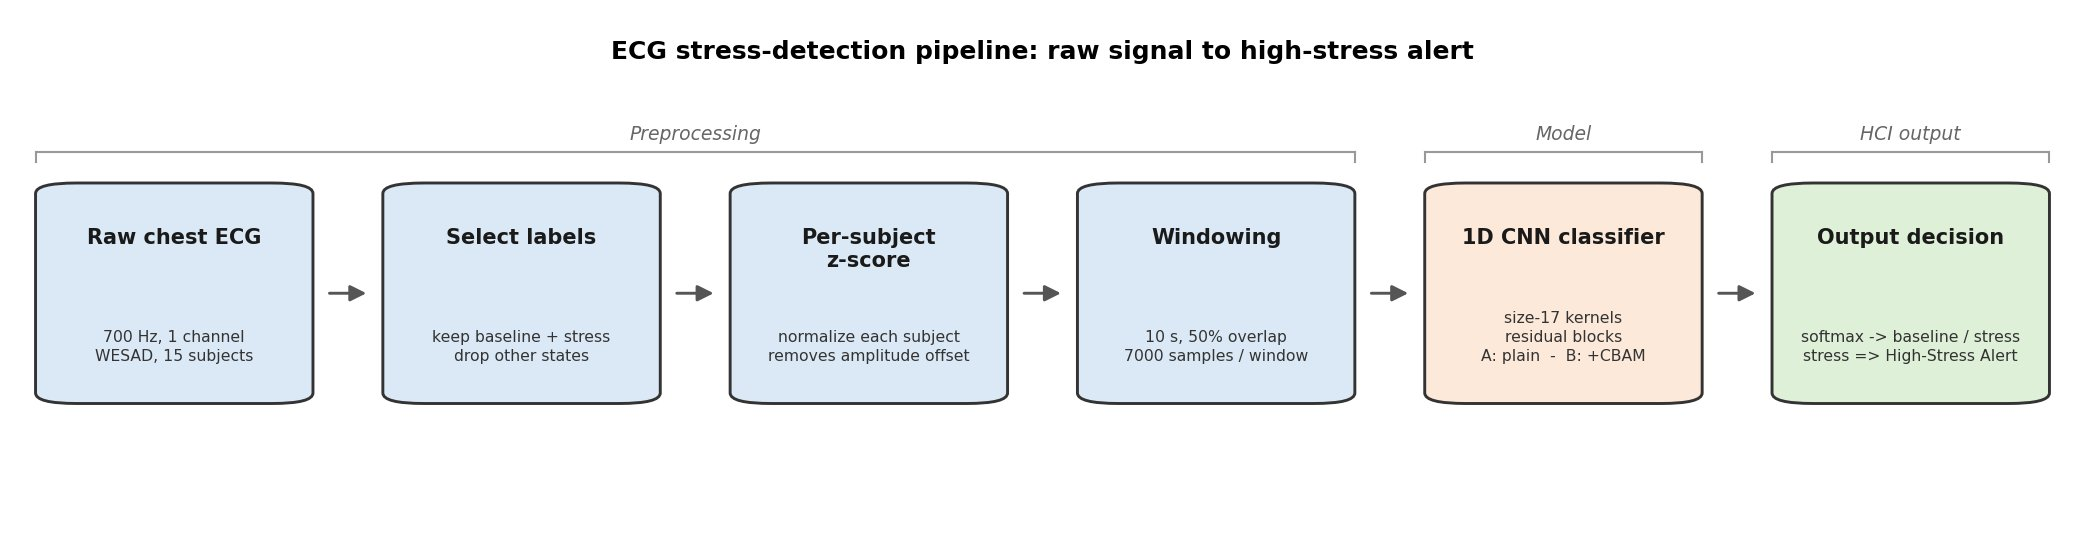
\includegraphics[width=\textwidth]{fig1_pipeline.png}
\caption{End-to-end pipeline of the ECG stress-detection system. Raw chest ECG
(700~Hz) is restricted to baseline and stress segments, normalized per subject,
and cut into overlapping 10-second windows (7000 samples). A 1D CNN classifies
each window as baseline or stress, and a stress prediction raises the high-stress
alert. Two model variants are compared: a plain 1D CNN (A) and the same network
with CBAM attention (B). Both are trained and evaluated with leave-one-subject-out
cross-validation.}
\label{fig:pipeline}
\end{figure*}

\textit{Signal cleaning.} We do not apply a heavy denoising filter to the ECG.
In Phase~1 we plotted the raw chest ECG and saw that the signal was clean and
that the heartbeat shape (the P-QRS-T complex) was clearly visible. Because the
signal is already clean, a strong filter would mostly remove useful information
instead of noise, so we feed the raw signal to the network and let it learn what
to use. The only cleaning we do is keep only the valid baseline and stress
segments.

\textit{Normalization.} ECG amplitude is different from person to person because
of body differences and sensor placement. If we did not correct for this, the
network could learn to recognize a person's amplitude instead of their stress
state. So we standardize the ECG separately for each subject with a z-score
(subtract that subject's mean and divide by that subject's standard deviation).
This removes amplitude and offset differences but keeps the shape of the
heartbeat, which is what carries the stress information. This directly handles
the inter-subject amplitude variation that is expected for wearable ECG.

\textit{Windowing.} A single ECG sample means nothing on its own, so we cut the
continuous signal into fixed windows. We use 10-second windows with 50\% overlap,
which at 700~Hz gives 7000 samples per window. We chose 10~s for two reasons.
First, stress is a sustained state, not a single heartbeat, so the window must be
long enough to contain several heartbeats and show the rhythm, and 10~s does this
easily. Second, the application is a real-time alert, and with 50\% overlap the
system produces a fresh decision every 5~s, which is responsive enough to catch a
sustained high-stress state without making the alert flicker on a single odd
beat. We make sure each window lies fully inside one condition, so no window
mixes baseline and stress.

\textit{Feature representation.} Because we want the network to learn from the
raw signal, the input is simply the 7000-sample window itself, arranged as one
channel over time. This matches a 1D CNN, which expects a one-dimensional signal
as its input. We do not compute spectrograms or any hand-crafted features.

\textit{Split strategy.} The most important choice in our evaluation is how we
split the data. We split by \textit{subject}, never by window. If windows from
the same person appeared in both training and testing, the model could score well
just by recognizing that person's heartbeat, and the result would be too
optimistic and would not reflect a new surgeon. To avoid this we use
leave-one-subject-out (LOSO) cross-validation: we train on 14 subjects and test on
the 1 subject left out, and we repeat this 15 times so that every subject is the
test subject exactly once. We then report the average performance across the 15
runs together with the standard deviation, which shows how much the result varies
from person to person. Inside each run, one of the 14 training subjects is also
held out as a small validation set used only to decide when to stop training; the
test subject is never looked at during training.

\subsection{Model Architecture}
Both models take a single 10-second window of raw ECG as input, shaped as one
channel of 7000 samples, and output two numbers (the scores for baseline and
stress). The backbone is a 1D convolutional network in the ResNet style. It
starts with a stem (one convolution that also halves the length, followed by
batch normalization, a ReLU activation, and max pooling), and then three
residual blocks. Each residual block has two convolutions with batch
normalization and a shortcut connection that adds the block's input to its
output, which is what lets the network be deep without the training breaking.
After the blocks, global average pooling turns each feature map into a single
number, a dropout layer reduces overfitting, and a final linear layer produces
the two class scores. The number of channels grows (32, 64, 128) while the
length shrinks, which is the usual trade in this kind of network.
Table~\ref{tab:arch} lists the layers.

All convolutions use a kernel size of 17. This is a large kernel on purpose: at
700~Hz, 17 samples cover enough of the signal for one filter to see a meaningful
piece of the heartbeat shape at once, which matches the idea (from the reviewed
paper \cite{reviewed} and our Phase~1 analysis) that the raw P-QRS-T shape is the
useful feature. The reviewed paper also reported that a larger kernel worked
better for this kind of ECG task, which supports our choice.

\begin{table}[t]
\caption{Backbone of Model~A. Model~B is identical but adds a CBAM block inside
each residual block. C\,$\times$\,L is channels\,$\times$\,length.}
\label{tab:arch}
\centering
\footnotesize
\begin{tabular}{|l|l|l|}
\hline
\textbf{Stage} & \textbf{Details} & \textbf{Output (C\,$\times$\,L)} \\
\hline
Input & raw ECG window & 1 $\times$ 7000 \\
\hline
Stem & Conv(k17,s2), BN, ReLU, MaxPool & 32 $\times$ 1750 \\
\hline
Res block 1 & 2$\times$Conv(k17) + shortcut & 32 $\times$ 1750 \\
\hline
Res block 2 & 2$\times$Conv(k17,s2) + shortcut & 64 $\times$ 875 \\
\hline
Res block 3 & 2$\times$Conv(k17,s2) + shortcut & 128 $\times$ 438 \\
\hline
Head & avg pool, dropout, linear & 2 \\
\hline
\end{tabular}
\end{table}

The two models differ in exactly one thing. Model~A is the plain backbone above.
Model~B is the same backbone with a Convolutional Block Attention Module (CBAM)
\cite{cbam} added inside every residual block, just before the shortcut is added.
CBAM has two small parts: channel attention, which learns which feature maps are
most useful, and spatial attention, which learns which time positions in the
window are most useful. The idea we took from the reviewed paper is that this
attention should help the network focus on the clean, informative part of the
heartbeat and ignore noise. Importantly, CBAM is very small: it adds only about
3000 parameters, around 0.5\% on top of the backbone, so any difference in the
results comes from the attention itself and not from a bigger model. Keeping
everything else identical between the two models is what makes the comparison
fair.

We train both models from scratch and do not use any pre-trained weights. There
is no standard pre-trained network for raw single-lead chest ECG the way there is
for natural images, and our input (one channel, 7000 samples) does not match
image models, so transfer learning would not apply cleanly here. The network is
also small enough to train quickly on our data, so training from scratch is the
simplest honest choice.

Table~\ref{tab:hparams} lists every hyperparameter with a short reason. A few are
worth highlighting. We use a weighted loss because baseline windows outnumber
stress windows about 1.8 to~1, and for a safety alert we would rather not
under-weight the stress class. We train with mixed precision and a small batch
size to stay within the 4~GB of GPU memory on the laptop we used. We use light
data augmentation (small changes to amplitude, a little noise, and a small time
shift) so the model relies on the heartbeat shape rather than memorizing
individual recordings. Finally, we pick the best epoch using the validation set
inside each fold and stop early if it stops improving, so we never report an
over-trained model.

\begin{table*}[t]
\caption{Hyperparameters and the reason for each. The last two rows apply to
Model~B only.}
\label{tab:hparams}
\centering
\footnotesize
\begin{tabular}{|l|l|p{11cm}|}
\hline
\textbf{Hyperparameter} & \textbf{Value} & \textbf{Reason} \\
\hline
Kernel size & 17 & Large kernel so one filter sees a full heartbeat shape; matches Phase~1 and the reviewed paper's finding that larger kernels help. \\
\hline
Base channels & 32, 64, 128 & Enough capacity to learn the shape while staying small for the 4~GB GPU. \\
\hline
Residual blocks & 3 & Deep enough to learn useful features, shallow enough to train on limited data. \\
\hline
Dropout & 0.5 & Strong regularization, because with only 15 subjects the model overfits quickly. \\
\hline
Optimizer & AdamW & Adam with weight decay; a stable and common choice. \\
\hline
Weight decay & 0.001 & Extra regularization to reduce overfitting to specific subjects. \\
\hline
Learning rate & 0.0003 & Small enough to train stably; a higher rate made the validation score jump around. \\
\hline
LR schedule & ReduceLROnPlateau ($\times$0.5) & Lower the learning rate when the validation score stops improving. \\
\hline
Batch size & 32 & Fits in 4~GB GPU memory; can be lowered to 16 or 8 if out of memory. \\
\hline
Max epochs & 40 & Upper limit only; training usually stops earlier. \\
\hline
Early stopping & patience 10 & Stop when validation stops improving and keep the best epoch, to avoid over-training. \\
\hline
Loss & weighted cross-entropy & Baseline outnumbers stress about 1.8 to~1; weighting makes missing a stress window cost more. \\
\hline
Mixed precision (AMP) & on & Lowers memory use so the model fits on the 4~GB GPU. \\
\hline
Augmentation & enabled & Small amplitude change ($\pm$20\%), Gaussian noise, and time shift ($\pm$0.2~s) so the model relies on heartbeat shape, not memorized recordings. \\
\hline
CBAM reduction ratio & 16 & Default from the CBAM paper; keeps the attention block tiny. \\
\hline
CBAM spatial kernel & 7 & Default from the CBAM paper. \\
\hline
\end{tabular}
\end{table*}

\section{Experimental Results}
We evaluate both models with leave-one-subject-out cross-validation (15 folds)
and report the average over the 15 held-out subjects. Because the two classes are
imbalanced, we use \textit{balanced accuracy} (the average of the per-class
accuracies) as the main score instead of plain accuracy, which can look high just
by predicting the majority class. We also report per-class precision, recall, and
F1, and we pay special attention to the stress class, because missing stress is
the error that matters for the alert.

Figure~\ref{fig:curves} shows the training and validation loss for a
representative fold of each model. In both cases the training loss falls steadily
while the validation loss reaches a minimum and then rises again, which is the
normal sign of over-fitting; the dashed line marks the epoch we keep (the lowest
validation loss). This figure is only meant to show the training behavior and the
early-stopping point; the actual comparison between the two models is in
Table~\ref{tab:results}, not here.

\begin{figure*}[t]
\centering
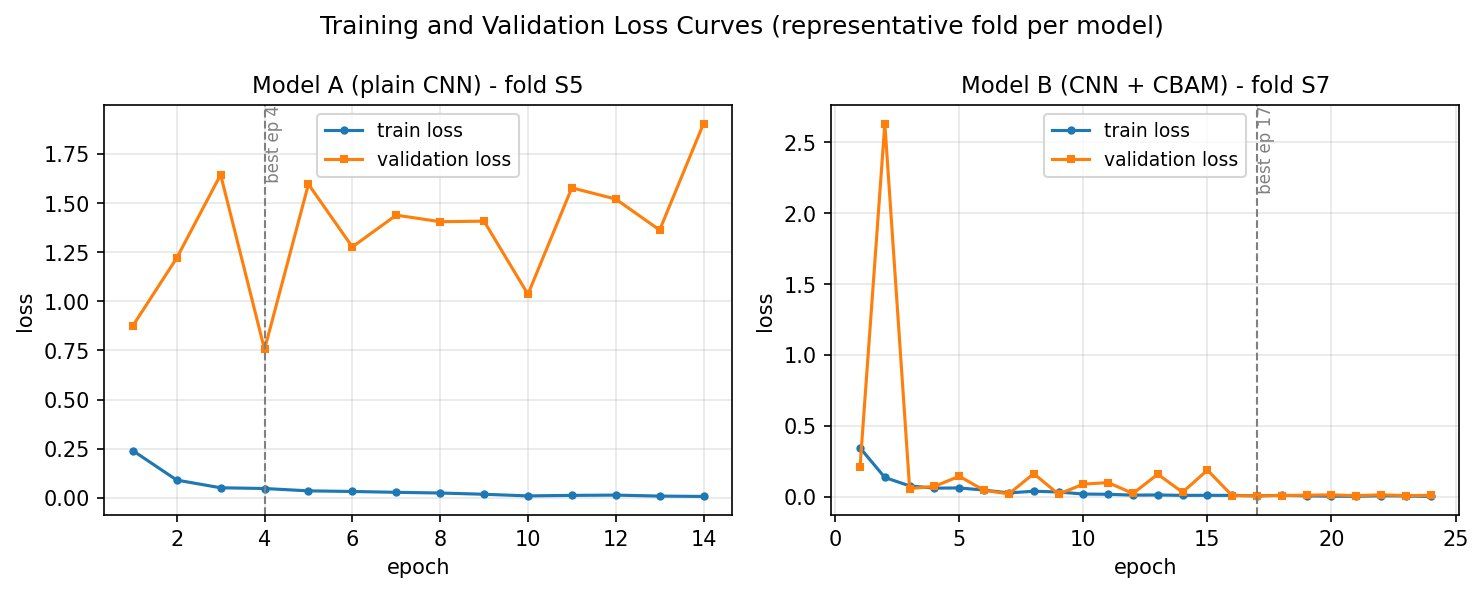
\includegraphics[width=0.82\textwidth]{fig2_curves.png}
\caption{Training and validation loss for a representative fold of each model
(Model~A: subject S5 held out; Model~B: subject S7 held out). The training loss
falls while the validation loss reaches a minimum and then rises (over-fitting);
the dashed line is the epoch kept by early stopping. This figure shows training
behavior only; the model comparison is in Table~\ref{tab:results}.}
\label{fig:curves}
\end{figure*}

Table~\ref{tab:results} reports the full per-class results for both models, and
Figure~\ref{fig:cm} shows the matching confusion matrices (all 15 held-out
subjects pooled together). The plain CNN (Model~A) is better on every measure. It
reaches a mean balanced accuracy of 0.829 against 0.729 for the CBAM model, and
the gap is largest exactly where it matters: Model~A correctly detects 93.9\% of
stress windows (stress recall), while Model~B detects only 75.3\%. In raw counts,
Model~A misses 121 stress windows while Model~B misses 488, about four times as
many. Both models raise a similar number of false alarms (Model~A predicts stress
on 972 baseline windows, Model~B on 1004), so the main difference is that CBAM
lets far more real stress slip through.

\begin{table}[t]
\caption{Per-class results for both models, pooled over the 15 LOSO folds. Higher
is better for every row.}
\label{tab:results}
\centering
\footnotesize
\begin{tabular}{|l|c|c|}
\hline
\textbf{Metric} & \textbf{Model A} & \textbf{Model B} \\
 & \textbf{(plain CNN)} & \textbf{(+ CBAM)} \\
\hline
Balanced accuracy (mean) & 0.829 & 0.729 \\
\hline
Balanced accuracy (std) & 0.197 & 0.197 \\
\hline
Plain accuracy (mean) & 0.799 & 0.726 \\
\hline
Baseline precision & 0.954 & 0.837 \\
\hline
Baseline recall & 0.723 & 0.713 \\
\hline
Baseline F1 & 0.822 & 0.770 \\
\hline
Stress precision & 0.656 & 0.597 \\
\hline
Stress recall & 0.939 & 0.753 \\
\hline
Stress F1 & 0.772 & 0.666 \\
\hline
\end{tabular}
\end{table}

\begin{figure*}[t]
\centering
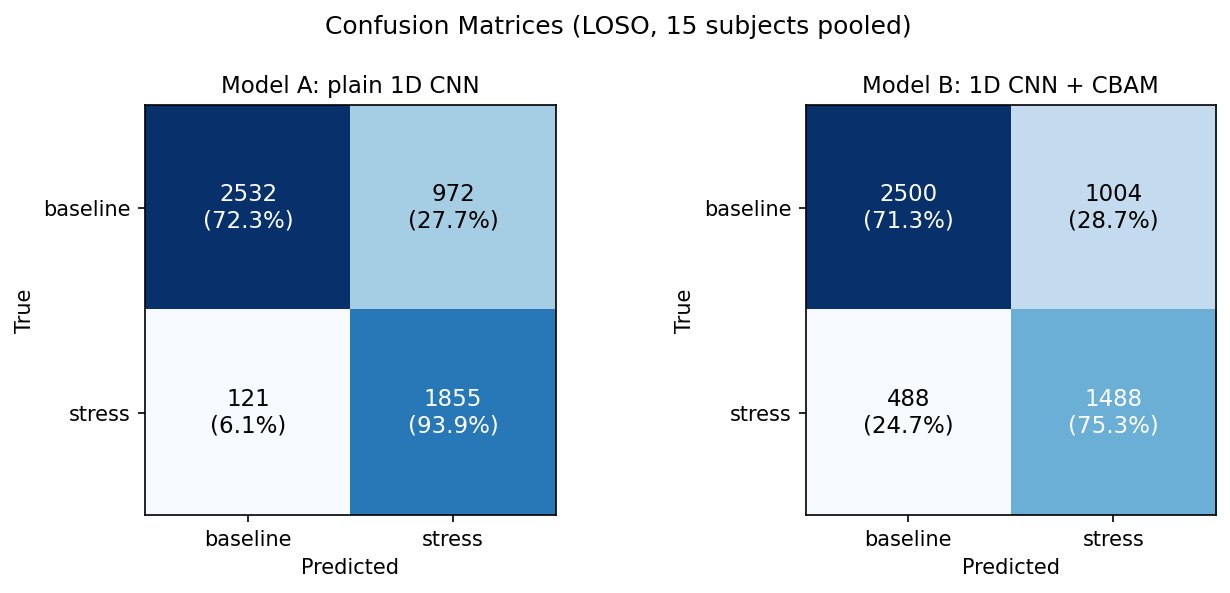
\includegraphics[width=0.82\textwidth]{fig3_confusion.png}
\caption{Confusion matrices for both models, pooled over all 15 held-out subjects
(rows: true class, columns: predicted; 0 = baseline, 1 = stress). The bottom-left
cell is missed stress: 121 windows (6.1\%) for Model~A versus 488 (24.7\%) for
Model~B.}
\label{fig:cm}
\end{figure*}

The standard deviation of the balanced accuracy is high (0.197 for both models),
and this is itself an important result rather than a flaw. Looking at the
individual folds, most subjects are classified very well (several above 0.98 for
Model~A) while a few collapse to about 0.50, which is chance level. In other
words, the system works very well for most unseen people and fails almost
completely for a small number of them. The most likely reason is that stress
shows up differently in different people: for some subjects the baseline and
stress ECG simply overlap, and no model trained on other people can separate two
states that look the same for that individual. We return to this in the HCI
assessment, because a system that is excellent on most users but unreliable on a
few is a safety concern, not just a number.

Finally, because the application is a real-time alert, we measured how long the
model takes to classify one window. On the laptop GPU, inference takes about
3.9~ms per window on average (about 5.8~ms in the worst case), and even on the CPU
it takes about 17~ms. This is far below the length of the window itself: a new
10-second window arrives every 5~s (with 50\% overlap), so the time to compute the
result is negligible compared with how often new data comes in. The real
responsiveness of the system is therefore set by the window design (a decision
every 5~s), not by the model, and both the GPU and the CPU are fast enough for
real-time use. We report Model~A's latency because it is our recommended model;
Model~B is essentially the same size and runs in a similar time.

\section{HCI Assessment}
A system that decides whether a surgeon is stressed can fail in several ways, and
in this application a wrong output is not just an inconvenience, it can be a
safety problem. Below we describe four failure modes using the template of
description, cause, HCI consequence, severity, and mitigation. The first three
come directly from our results.

\subsection{Failure Mode Analysis}

\textit{FM1 --- The system cannot separate stress from baseline for some
individuals.}
\textbf{Description:} for a few subjects the model performed at chance level
(balanced accuracy near 0.50 in the LOSO folds, for example S2 and S10), so for
those people it cannot reliably tell stress from calm.
\textbf{Cause:} inter-individual variation --- for these subjects the baseline and
stress ECG overlap, so a model trained on other people has no feature that
separates the two states (an out-of-distribution individual).
\textbf{HCI consequence:} for that surgeon the monitor is effectively broken: it
may stay silent during real stress or fire at random, while still looking like it
is working.
\textbf{Severity:} High --- a monitor that silently does not work gives false
reassurance during surgery, which is worse than having no monitor at all.
\textbf{Mitigation:} add a short per-surgeon calibration (record a known calm and
a known stressed sample, then set a personal threshold or fine-tune), and report
``not calibrated / low confidence'' instead of a confident guess.

\textit{FM2 --- Missed stress (false negative).}
\textbf{Description:} even the better model labels about 6\% of true stress
windows as baseline (121 of 1976; with CBAM this rose to about 25\%), so it
sometimes fails to raise the alert when the surgeon is stressed.
\textbf{Cause:} windows close to the decision boundary and mild stress responses,
with the threshold at the default 0.5.
\textbf{HCI consequence:} the assistant is not prompted during a genuine
high-stress moment --- the exact situation the system exists for is the one it
misses.
\textbf{Severity:} High --- missing stress is the most dangerous error for this
application.
\textbf{Mitigation:} lower the stress threshold to trade a few more false alarms
for fewer misses, favoring sensitivity over precision for a safety alert.

\textit{FM3 --- False alarm during calm periods (false positive).}
\textbf{Description:} the model predicts stress on about 28\% of baseline windows
(972 of 3504), so the alert sometimes fires when the surgeon is calm.
\textbf{Cause:} short signal changes that look like arousal, plus the weighted
loss deliberately leaning toward the stress class.
\textbf{HCI consequence:} alert fatigue --- if the alert fires too often when
nothing is wrong, the surgeon or assistant learns to ignore it, including when it
is right.
\textbf{Severity:} Medium --- a single false alarm is not dangerous, but repeated
false alarms erode trust and can cause real alerts to be ignored.
\textbf{Mitigation:} only raise the alert when stress persists across several
consecutive windows (temporal smoothing) rather than on a single window.

\textit{FM4 --- Confident output on a corrupted (out-of-distribution) signal.}
\textbf{Description:} when the ECG is corrupted by heavy motion, electrode
movement, or the noisy transition periods we saw in Phase~1, the model still
outputs a confident baseline or stress label.
\textbf{Cause:} out-of-distribution input --- the network was trained on clean
labeled segments and has no ``reject / unknown'' option, so it extrapolates.
\textbf{HCI consequence:} a confidently wrong reading during fast movements or
instrument changes, which are exactly the moments when stress may be high.
\textbf{Severity:} High --- a confident wrong output at a critical moment is worse
than showing nothing.
\textbf{Mitigation:} add a signal-quality check that rejects or down-weights noisy
windows and shows an ``uncertain / poor signal'' state instead of forcing a binary
decision.

\subsection{Nielsen's Heuristics}
Table~\ref{tab:nielsen} maps several of Nielsen's usability heuristics to this
system. The common theme is that the interface must stay minimal and honest about
its own uncertainty, because anything that demands attention during the critical
phase would make the cognitive tunneling worse, not better.

\begin{table}[t]
\caption{Selected Nielsen usability heuristics and how they apply to the alert.}
\label{tab:nielsen}
\centering
\footnotesize
\begin{tabular}{|p{2.4cm}|p{4.9cm}|}
\hline
\textbf{Heuristic} & \textbf{Application to our system} \\
\hline
Visibility of system status & Show the current state and a confidence level, and clearly flag poor signal quality or an uncalibrated user instead of a bare yes/no. \\
\hline
Match with the real world & Map the output to a concrete action (prompt an assistant, suggest a micro-break) rather than showing raw probabilities. \\
\hline
Error prevention & Require stress to persist over several windows before alerting, to avoid reacting to a single noisy reading. \\
\hline
Recognize and recover from errors & Let the team see why an alert fired and acknowledge or dismiss it, so a wrong alert is corrected quickly. \\
\hline
Aesthetic and minimalist design & Use a subtle, non-intrusive cue; a busy display would compete for attention and worsen cognitive tunneling. \\
\hline
\end{tabular}
\end{table}

\section{Conclusion}
We built a real-time stress monitor for surgeons that reads raw chest ECG and
decides between calm and stressed, which would drive a high-stress alert. We
implemented the full pipeline (per-subject normalization, 10-second windowing,
and a 1D CNN with large kernels and residual connections) and compared a plain
CNN with a CBAM version, evaluating both honestly with leave-one-subject-out
cross-validation.

The plain CNN is our recommended system. It reached a mean balanced accuracy of
0.829 and detected about 94\% of stress windows on subjects it had never seen,
with inference fast enough (about 4~ms per window) for real-time use. Adding CBAM
did not help: it lowered balanced accuracy to 0.729 and missed about four times
as many stress windows. The most likely reasons are that our signal was already
clean (so there was little noise for attention to suppress) and that attention
needs more data than 15 subjects to learn a general rule. This is an honest
negative result, and a useful one: here the simpler model is both more accurate
and safer, and adding complexity was not an improvement.

The main limitation is that performance varies a lot between people: the system
is excellent for most subjects but drops to chance level for a few whose calm and
stressed ECG overlap. For a safety system this matters more than the average
score.

For Phase~3 we would: (1) add a short per-surgeon calibration so the model adapts
to each person and reduces the chance-level failures; (2) add a signal-quality
check and an ``uncertain'' state so the system does not give confident wrong
answers on noisy input; (3) apply temporal smoothing so the alert responds to
sustained stress rather than single windows; and (4) move from a fixed threshold
to one tuned for high stress recall, since missing stress is the costliest error.
Together these target the failure modes above and would make the alert safer to
use in a real operating room.

\begin{thebibliography}{00}

\bibitem{reviewed} T. Fan, S. Qiu, Z. Wang, H. Zhao, J. Jiang, Y. Wang, J. Xu,
T. Sun, and N. Jiang, ``A new deep convolutional neural network incorporating
attentional mechanisms for ECG emotion recognition,'' \textit{Computers in
Biology and Medicine}, vol. 159, art. 106938, 2023.

\bibitem{cbam} S. Woo, J. Park, J.-Y. Lee, and I. S. Kweon, ``CBAM: Convolutional
block attention module,'' in \textit{Proc. European Conf. Computer Vision
(ECCV)}, 2018, pp. 3--19.

\bibitem{resnet} K. He, X. Zhang, S. Ren, and J. Sun, ``Deep residual learning
for image recognition,'' in \textit{Proc. IEEE Conf. Computer Vision and Pattern
Recognition (CVPR)}, 2016, pp. 770--778.

\bibitem{hannun} A. Y. Hannun, P. Rajpurkar, M. Haghpanahi, G. H. Tison,
C. Bourn, M. P. Turakhia, and A. Y. Ng, ``Cardiologist-level arrhythmia detection
and classification in ambulatory electrocardiograms using a deep neural
network,'' \textit{Nature Medicine}, vol. 25, no. 1, pp. 65--69, 2019.

\bibitem{wesad} P. Schmidt, A. Reiss, R. Duerichen, C. Marberger, and K. Van
Laerhoven, ``Introducing WESAD, a multimodal dataset for wearable stress and
affect detection,'' in \textit{Proc. 20th ACM Int. Conf. Multimodal Interaction
(ICMI)}, 2018, pp. 400--408.

\bibitem{kiranyaz} S. Kiranyaz, T. Ince, and M. Gabbouj, ``Real-time
patient-specific ECG classification by 1-D convolutional neural networks,''
\textit{IEEE Trans. Biomedical Engineering}, vol. 63, no. 3, pp. 664--675, 2016.

\end{thebibliography}

\end{document}
